\documentclass{beamer}
\usepackage{pgf, pgffor}
\usepackage{bibentry}
\usepackage{textcomp}
\usepackage{graphicx} 
\usepackage{listings}
\usepackage{xcolor}
\usepackage{color}
\usetheme{Madrid}
\usepackage{lstlinebgrd} % see http://www.ctan.org/pkg/lstaddons


\definecolor{codegreen}{rgb}{0,0.6,0}
\definecolor{codeDarkGreen}{rgb}{0,0.3,0}
\definecolor{codegray}{rgb}{0.5,0.5,0.5}
\definecolor{codepurple}{rgb}{0.58,0,0.82}
\definecolor{backcolour}{rgb}{0.95,0.95,0.92}

\lstdefinestyle{CppCodeStyle}{
    backgroundcolor=\color{backcolour},   
    commentstyle=\color{codegray},
    keywordstyle=\color{blue},
    numberstyle=\tiny\color{codegray},
    stringstyle=\color{codepurple},
    basicstyle=\footnotesize,
    breakatwhitespace=false,         
    breaklines=true,                 
    captionpos=b,                    
    keepspaces=true,                 
    numbers=left,                    
    numbersep=5pt,                  
    showspaces=false,                
    showstringspaces=false,
    showtabs=false,                  
    tabsize=2,    
	morekeywords={JNIEnv, jobject, jstring, jmethodID, jclass, jthrowable},        
	% keywords with a different color    
    classoffset=1, % starting new class
    morekeywords={JNIEXPORT, JNICALL},
    keywordstyle=\color{codeDarkGreen},
    classoffset=0, % reset class
}

\lstdefinestyle{JavaCodeStyle}{
    backgroundcolor=\color{backcolour},   
    commentstyle=\color{codegray},
    keywordstyle=\color{blue},
    numberstyle=\tiny\color{codegray},
    stringstyle=\color{codepurple},
    basicstyle=\footnotesize,
    breakatwhitespace=false,         
    breaklines=true,                 
    captionpos=b,                    
    keepspaces=true,                 
    numbers=left,                    
    numbersep=5pt,                  
    showspaces=false,                
    showstringspaces=false,
    showtabs=false,                  
    tabsize=2,
}



%\usetheme{Madrid}[rounded][shadow=false]

\title{Android Insider Attacks} 
\author{David Goeth} 
\institute[]{University of Passau \newline 
Advanced seminar: Real Life Security \newline
WS 2017/2018}
\date{January 19, 2018} 


\begin{document}

%\setbeamertemplate{Madrid}[rounded][shadow=true]

\begin{frame}
\titlepage % Print the title page as the first slide
\end{frame}

%\maketitle

%\begin{frame}{}
%\begin{block}{}
%	From the "Call for Papers" Presentation Slides\footnotemark
%\end{block}
%   \begin{itemize}
%   	\item Android apps can include shared libraries with native code
   	%\item Shared libraries executed alongside byte code in the same address space
   	%\item What if the native library is not trusted? 
%   	\item Develop scenario for vulnerable (Java-bytecode) app
%   	\item Write malicious sample library demonstrating attacks
%   	\item Analyze the underlying reasons making these attacks possible
%   \end{itemize}
   
   % This statement requires citation \cite{AndroidNdkIntro}
   
%   \footnotetext{GeneralInfo\_Deadlines.pdf, slide 9:\newline
%   \url{https://studip.uni-passau.de/studip/sendfile.php?type=0&file%\_id=12ff93b0f8a63b7c21889a9ddd7971bf&file_name=GeneralInfo\_Deadlines.pdf}}
%\end{frame}


\begin{frame}{Overview}
\tableofcontents
\end{frame}


\section{Motivation}
\begin{frame}{Motivation}
    \begin{itemize}
    \item Vast amount of data in the fields of medicine
    \item Data is heterogeneous (e.g. using different file formats)
    \item Data isn't easily accessible and needs lots of tools
    
    \item Research and health care institutions would benefit from a unique view of data \cite{Raghupathi2014}:
    \begin{itemize}
    	\item Lower Costs
    	\item Detecting diseases at early stages
    	\item Simplified collaboration
    	\item Health care fraud detection
    \end{itemize}
    \end{itemize}
\end{frame}

\def \data_integration_title{Data Integration}

\section{Data Integration}
\begin{frame}{\data_integration_title}
    \begin{itemize}
    \item Data integration addresses the integration of data sources into one information system \cite{DBLP:books/dp/LeserN2006}
    \item Unified view of the data
    \item Uses a global schema local data source schemas have to be translated to.
    \item Types of integration: Materialized, Virtual, Hybrid
    %\item Wrapper: Takes care of the communication between the data source and the integrated system

\end{itemize}    
\end{frame}

\begin{frame}{Heterogeneous Data Sources}
    \begin{itemize}
    \item Data sources providing not the same methods, models  and structures for accessing their data
    \item Technical: Query language, exchange format, communication protocol,...
    \item Syntactic: Number formats, character encoding, tab vs. comma separated values in CSV files  $\Rightarrow$ In general: Technical differences in the presentation of information
    \item Data model: relational, object-oriented, graph-based,...
    \item Semantic: Differences in the interpretation/meaning of the data
    \item Structural: Schemas are different though they are semantically equal 
    \end{itemize}
\end{frame}

\begin{frame}{Ontology}
    \begin{itemize}
    \item Defines the concepts, relationships, and other distinctions being relevant for modeling a domain \cite{9780387355443}.
    \item Operates on the semantic level rather than on the logical/physical one.
    \item Independent from lower data models
    \item Can be used to solve semantic heterogeneity: Logical Inference
    \item Suitable for integrating heterogeneous data sources 
    \end{itemize}
\end{frame}



\section{Dataspace}
\begin{frame}{Dataspace}
\begin{itemize}
    \item New abstraction of data management \cite{Franklin:2005:DDN:1107499.1107502}
    \item Data to be managed rarely stored using a single data model
    \item Supports all kind of data rather than only a few
    \item Provides tools allowing a tighter data integration process when required
    \item Difference to a Data Integration System (DIS): Data coexistence. DIS needs a semantic integration process before providing any services.
    \item Pay-as-you-go integration
    \item Multimedia dataspace model\cite{6167826}
    \begin{itemize}
    	\item classes, objects and relations
    	\item Similarity relations
    	\item Dataspace views
    	\item Meets requirements for multimedia data
    \end{itemize}
\end{itemize}
\end{frame}



\section{Implementation}
\begin{frame}
\begin{figure}[H]
	\begin{center}
	\vspace*{-0.35cm}
		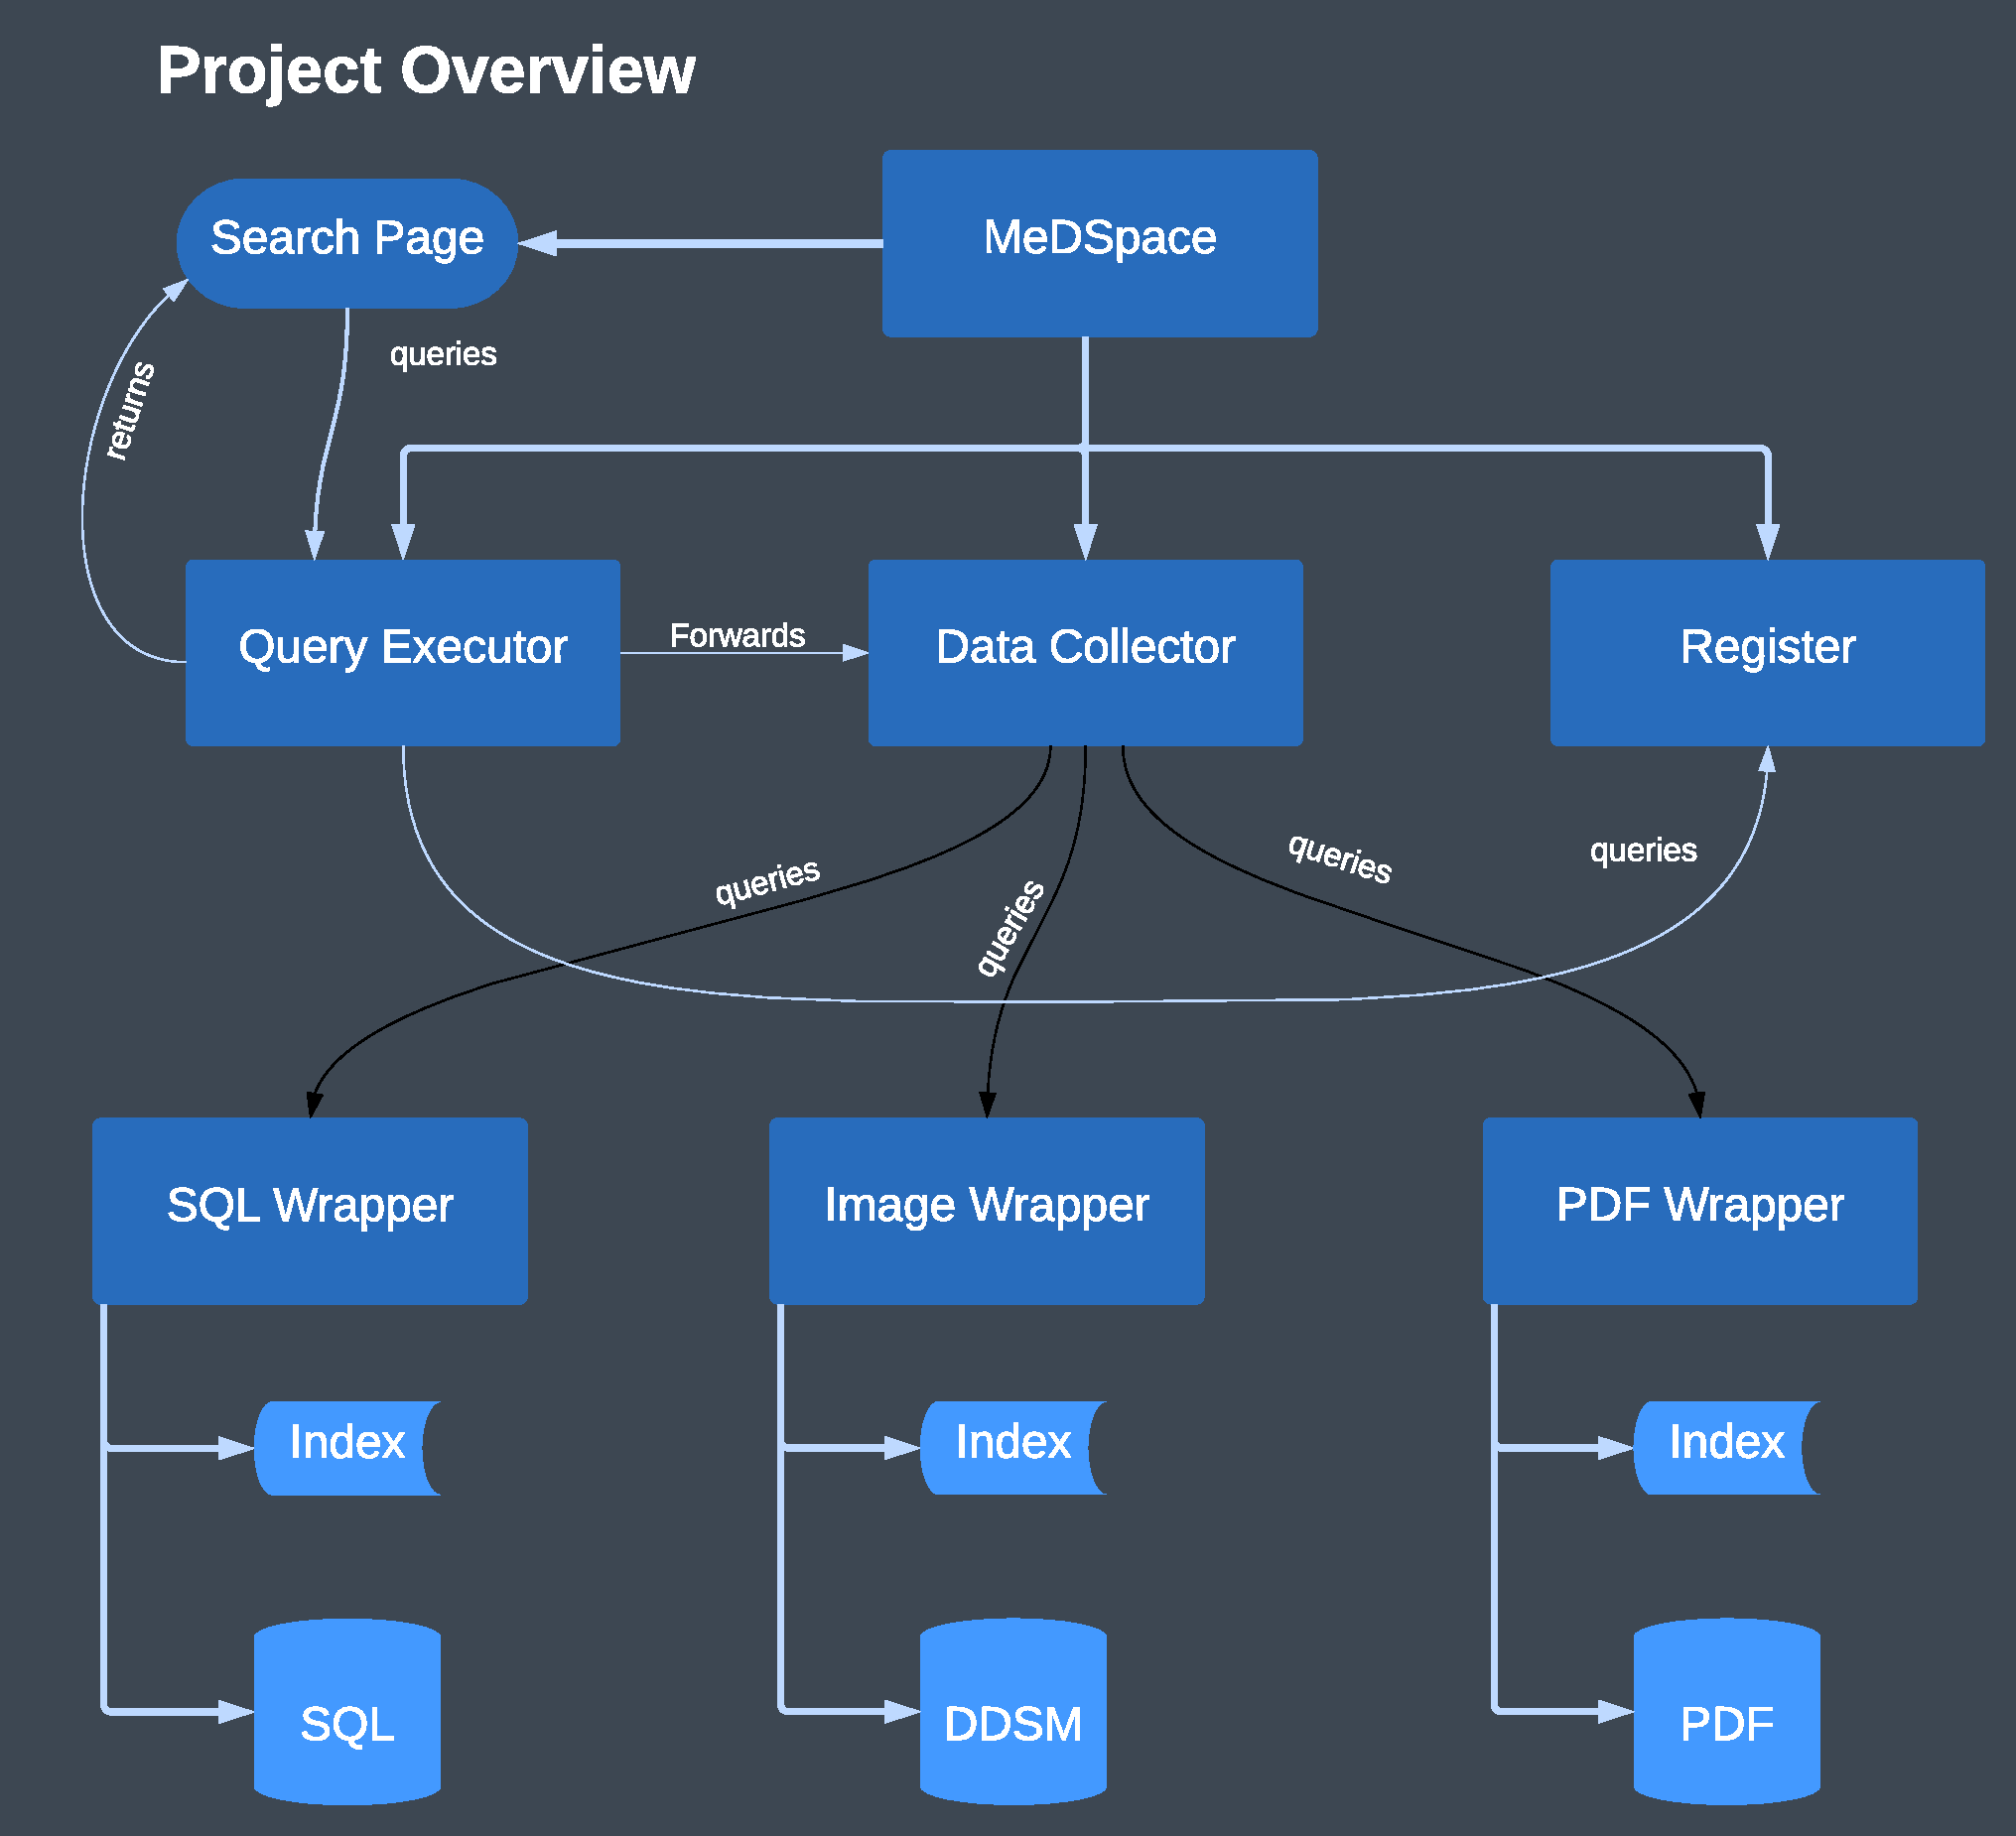
\includegraphics[scale=0.3]{figures/MeDSpace-Overview.pdf}
	\end{center}
	\label{MeDSpaceOverview}
\end{figure}
\end{frame}

\begin{frame}{Implementation}{Project goals}
    \begin{itemize}
    \item Setting up three heterogeneous data sources containing medical data about breast cancer (Relational, Images, PDF Files)
    \item Implementing wrappers adding keyword search functionality to the data sources
    \item Wrappers register themselves to the Register
    \item Convert data of search results to RDF
    \item All data sources can be queried through an unified user interface  
    \end{itemize}
\end{frame}

\begin{frame}{RDF}
    \begin{itemize}
    \item Resource Description Framework (RDF) \cite{rdf11concepts}
    \item Graph-based abstract data model 
	\item Facilitates merging data expressed in different schemas
    %\item Allows mixing of structured and semi-structured data    
    %\item Used as data representation format)
    %$\Rightarrow$  IRIs enables to hold heterogenous data in one data set
    %\item Follows Linked Open Data recommendation \textcolor{red}{TODO}
    \item RDF4J (formerly Sesame) framework used in the thesis' project \cite{RDF4J}
    \end{itemize}
\end{frame}

\begin{frame} {RDF}
\begin{figure}[H]
	\begin{center}
		
\includegraphics[scale=0.75]{figures/rdf-graph.pdf}
	\end{center}
	\caption{Connection between two nodes (Subject, Object) forming an RDF Triple
	\footnotemark
	}
	\label{RdfTriple}
\end{figure}
\begin{itemize}
	\item Three kinds of nodes: IRI, literals, blank nodes
    \item Relations between nodes are specified by predicates 
    \item Predicates are IRIs themselves
    \item Web Ontology Language (OWL) can be used to define ontologies using rdf \cite{owlSpec}
\end{itemize}

\footnotetext{\url{https://www.w3.org/TR/rdf11-concepts/rdf-graph.svg}}
\end{frame}

\begin{frame}{Wrapper (general)}
\begin{itemize}
    \item Proxy for a datasource
    \item Transforms an incoming dataspace query into a query the wrapped datasource understands.
    \item Offers its services through REST services, powered by the Play framework \cite{Play}
    \item Registers and deregisters autonomously to the dataspace 
    \item Has to offer at least a keyword search query service
    %\item XML configuration file using JAXB \cite{JAXB} 
    \item Apache Lucene used to offer fulltext search functionality \cite{LuceneCore}
    \item Keyword search currently only supports OR boolean operator
    \item On startup index for the keyword search service is created
    %\begin{itemize}
    %	\item Fetch data from the datasource
    %	\item index them using apache lucene
    %	\item store index 
    %\end{itemize}
\end{itemize}
\end{frame}

\begin{frame}{SQL Wrapper}
    \begin{itemize}
    \item Sample data used from Schmidbauer's PDGF \cite{SchmidbauerBachelorThesis}
    \item sql data is translated into rdf equivalent using Bizer's D2R Map language \cite{D2rMap_aDatabaseToRdfMappingLanguage}
    \item relational to rdf mappings are defined in seperate configuration file
    \end{itemize}
\end{frame}

\begin{frame}{Image Wrapper}
    \begin{itemize}
    \item Digital Database for Screening Mammographyc(DDSM)\cite{DDSM}
    \item Mammography Images used to seek for breast cancer
    %\item A case folder contains source images, overlay and case meta data
    %\item  \textcolor{red}{TODO: Example of a case folder structure or an except from the metadata?}
    \item DDSM-Utility used to convert (old) JPEG1 files to PNG \cite{DDSM_UTILITY} 
    %\item RDF Transformation rules defined in own configuration file
    \end{itemize}
\end{frame}

\begin{frame}{PDF Wrapper}
    \begin{itemize}
    \item Apache PDFBox \cite{PDFBox} for extracting unstructured text content from pdf files.
    \item The pdf files were formerly created using Schmidbauer's medical sql data set \cite{SchmidbauerBachelorThesis}
    %\item Configuration file defining RDF transformation rules (cf. Image Wrapper)
    \end{itemize}
\end{frame}

\begin{frame}{MeDSpace}
    \begin{itemize}
    \item Responsible for managing registered datasources
    \item Provides user interface for executing search queries
    \item User Interface and REST services powered by Play framework \cite{Play}
    \item Keyword search queries are forwarded to each datasource. The result is collected by the 
    data-collector module
    \item Query results are (temporarily) stored in separate RDF repositories
    %\item In final implementation: Search results get cached. Useful for quick access and useful for further data integration
    \end{itemize}
\end{frame}


\section{Improvements and Outlook}
\begin{frame}{Improvements and Outlook}
    \begin{itemize}
    \item Query caching
    \item Incremental (Pay-as-you-go) data integration
	\item Inferring knowledge using ontologies    
    \item Query language for multimedia data \cite{6214725}
    \end{itemize}    
\end{frame}

\begin{frame}[allowframebreaks]{References}
    %\bibliographystyle{ieeetr}
    \bibliographystyle{amsalpha}
    \bibliography{bib}
    %\addcontentsline{toc}{frame}{\bibname}
\end{frame}
\end{document}
